

%\documentclass[aps,twocolumn,secnumarabic,balancelastpage,amsmath,amssymb,nofootinbib, floatfix]{revtex4}
\documentclass[aps,twocolumn,secnumarabic,balancelastpage,amsmath,amssymb,nofootinbib,floatfix]{revtex4-1}

%%%%%%%%%%%%%%%%%%%%%%%%%%%%%%%%%%%%%%%%%%%%%%%%%%%%%%%%%%%%%%%%%%%
% N.B.:  Different computers have different packages installed.  
%        To compile this template in the current Athena 
%        environment, REVTeX 4.1 must be used.  To use the older
%        REVTeX 4, switch which documentclass line above is 
%        commented out above. There are ``bad'' distributions of
%        LaTeX for Windows available on the internet which may 
%        cause users to struggle unjustifiably with REVTeX 4.1.
%
%        If you are unable to compile the template at all, you
%        may need to update your LaTeX packages. (Alternatively, if 
%        your LaTeX distribution includes only the older RevTEX 4,
%        then try changing the documentclass line above. In particular,
%        this approach solves a common compilation problem for users of
%        the TeXWorks editor on Windows, which presents erroneously as a
%        error in the bibliography file.) Don't hesitate to speak 
%        with your section instructor or a TA if you're having 
%        issues getting this template to compile.
%%%%%%%%%%%%%%%%%%%%%%%%%%%%%%%%%%%%%%%%%%%%%%%%%%%%%%%%%%%%%%%%%%%

%%%%%%%%%%%%%%%%%%%%%%%%%%%%%%%%%%%%%%%%%%%%%%%%%%%%%%%%%%%%%%%%%%%
% = Explanation of documentclass options =
%
% aps, prl stand for American Physical Society and Physical 
%     Review Letters respectively.
% twocolumn permits two columns, of course.
% nobalancelastpage doesn't attempt to equalize the lengths of 
%     the two columns on the last page  as might be desired in a 
%     journal where articles follow one another closely.
% amsmath and amssymb are necessary for the subequations 
%     environment among others. These functionalities can
%     also be added use the usepackage function described below,
%     but REVTeX conveniently includes them as documentclass
%     options.
% secnumarabic identifies sections by number to aid electronic 
%     review and commentary.
% nofootinbib forces footnotes to occur on the page where they are
%      first referenced and not in the bibliography.
% floatfix attempts to help LaTeX decide where to place ``floats'',
%      like figures and plots, when it gets stuck and can't decide
%      by it's normal algorithm.
% REVTeX 4.1 is a set of macro packages designed to be used with 
%      LaTeX 2e. REVTeX is well-suited for preparing manuscripts 
%      for submission to APS journals.
%
% = Other documentclasses =
%
% The 'revtex4' and 'revtex4-1' documentclasses are somewhat 
%    specialized for making documents in the style of the APS
%    journals. For a more standard or generic looking LaTeX paper,
%    you could try any of the built-in documentclasses, in 
%    particular 'article' or 'report'. Someday, you may try to use 
%    the 'mitthesis'  documentclass available for download from the 
%    MIT Libraries. The vast majority of source code written for 
%    one documentclass should work just fine in any other, but 
%    occasional quirks arise. For example, some documentclasses 
%    disagree on whether the abstract declaration should come 
%    before or after the \begin{document} declaration.
% 
%%%%%%%%%%%%%%%%%%%%%%%%%%%%%%%%%%%%%%%%%%%%%%%%%%%%%%%%%%%%%%%%%%%

%% Now, include some packages which provide new commands that 
%% extend LaTeX's capabilities. Note that the nearly-essential
%% AMS math packages were added already as documentclass options
%% for REVTeX, but could have been added here using 
%% \usepackage{amsmath}, etc. The pacakges below are commonly 
%% useful, but there are many, many more available to solve a 
%% multitude of typesetting quandries (google your problem), 
%% and you  probably have the necesary packages installed on your
%% system already. Among the examples listed below, this sample
%% document only actually makes use of the 'graphicx', 'bm', 
%% and 'hyperref' pacakges, so the others are commented out for
%% tidyness.


\usepackage{graphicx}      % tools for importing graphics
\usepackage{physics}
\usepackage{tabularx}
\usepackage{booktabs}
%\usepackage{lgrind}        % convert program code listings to a form 
                            % includable in a LaTeX document
%\usepackage{xcolor}        % produces boxes or entire pages with 
                            % colored backgrounds
%\usepackage{longtable}     % helps with long table options
%\usepackage{epsf}          % old package handles encapsulated postscript issues
\usepackage{bm}            % special bold-math package. usge: \bm{mathsymbol}
%\usepackage{asymptote}     % For typesetting of mathematical illustrations
%\usepackage{thumbpdf}
\usepackage[colorlinks=true]{hyperref}  % this package should be added after 
                                        % all others.
                                        % usage: \url{http://web.mit.edu/8.13}


%%%%%%%%%%%%%%%%%%%%%%%%%%%%%%%%%%%%%%%%%%%%%%%%%%%%%%%%%%%%%%%%%%%
% And now, begin the document...
%%%%%%%%%%%%%%%%%%%%%%%%%%%%%%%%%%%%%%%%%%%%%%%%%%%%%%%%%%%%%%%%%%%

\begin{document}
\title{Measuring the Electron Charge $e$ using Shot Noise}
\author{Ethan Suresh}
\email{easuresh@mit.edu}
\author{Max Misterka}
\email{misterka@mit.edu}

\date{\today}
\affiliation{MIT Department of Physics}


\begin{abstract}
We measure the electron charge $e$ using the phenomenon of shot noise, an inherent source of current fluctuations in a conductor arising from the granular nature of charge. Shot noise follows Poisson statistics, in which the mean-squared current fluctuation is proportional to the average DC current through the conductor. An uncorrelated source of photoelectrons is generated using a variable-intensity lamp and passed through an amplifier-filter measurement chain to magnify the shot noise signal to a tractable level. By measuring the mean-squared shot noise current at a variety of lamp intensities, we observe a robust linear relationship consistent with the theory of shot noise. We obtain $e = \left( 1.858 \pm 0.008_{\rm stat} \pm 0.019_{\rm sys} \right) \times 10^{{-19}}\,\text{C}$, which deviates from the accepted value by approximately $12.63\,\sigma$. We are therefore unable to obtain an accurate measurement of the electron charge, and further investigation is required to identify the systematic effects present in our apparatus.
    
\end{abstract}

\maketitle




%%%%%%%%%%%%%%%%%%%%%%%%%%%%%%%%%%%%%%%%%%%%%%%%%%%%%%%%%%%%%%%%%%
\section{Introduction}

In the early 20th century, the nature of electric current was established to be granular, being composed of discrete particles carrying charge $e$. The prediction and experimental observation of shot noise provided a precise and direct method to measure the charge of the electron, lending credence to the granular nature of electric current. In the theory of shot noise, electrons are approximated as unit impulses of current arriving at a given point in the circuit, the detector, at times $T_k$, denoted $i(t-T_k)$ \cite{mit_johnson_shot_noise_2023}. Their arrival at the detector is assumed to be statistically independent, given that the current generation source, such as a battery or photodiode, is itself random. When a DC voltage $V$ is applied to a conductor, the net current or charge per unit time at the detector $I$ will achieve an average value given by Ohm's Law: $V = IR$, but will fluctuate about this time average due to variations in the number of electrons passing through the detector. The rate of charge arriving at the detector per unit time interval can be modeled as a Poisson distribution with mean and variance $I_{\text{avg}} = Ke$ \cite{mit_johnson_shot_noise_2023}. Additionally, the mean squared current $\langle I^2 \rangle$ yields important information about the fluctuation about the average value.

While $I_{\text{avg}}$ is straightforward to measure as a voltage  using a large resistance value $R_F$,  the rate $K$ is difficult to measure, and the typical shot noise voltage fluctuation is very small, often on the order of microvolts \cite{mit_johnson_shot_noise_2023}. Amplifying the shot noise can yield experimentally tractable values of  $\langle I^2 \rangle$. Suppose that the resistor $R_F$ is connected to an amplifier-filter apparatus which applies a frequency-dependent gain $g(f)$ on each Fourier component of the input time-varying signal $V(t) = I(t)R_F$. 

Summing over all frequencies in quadrature, the net squared gain $G$ can be found as 

\begin{equation}
    G = \int_0^{\infty} g(f)^2 \dd f
\end{equation}

which represents the overall gain of the experimental apparatus. A relation between the mean squared current and the DC current can be established \cite{mit_johnson_shot_noise_2023}: 

\begin{equation}
    \langle I^2 \rangle_{\rm shot} = 2e\, G\, I_{\rm avg} + C
    \label{eq:shot-noise}
\end{equation}

where $C$ is a constant offset arising from background noise sources such as Johnson noise and environmental electromagnetic interference. Using Eq.~\eqref{eq:shot-noise}, an experimental apparatus with known gain $G$ and measurements of $I_{\rm avg}$ and $\langle I^2 \rangle_{\rm shot}$ can be used to determine the electron charge $e$.

\section{Experimental Methods}

We describe how the overall measurement and calibration of $\langle I^2 \rangle_{\rm shot}$, $I_\text{avg}$, and $G$ are achieved using the apparatus described in Fig. \ref{fig:apparatus}. The current source, which is assumed to produce electrons at statistically independent times, is generated by a battery-powered lamp of variable intensity illuminating a photodiode with a stream of photons which excite individual electrons into the conduction band. The PIN-10D silicon photodiode is operated in a \emph{photoconductive} (reverse-biased) mode, with a bias of $-27$ V, making it more responsive to incoming photons \cite{osi_optoelectronics_photoconductive_photodiodes}. The resulting current is then converted into a voltage across a precision feedback resistor $R_F \approx 475 \ \text{k}\Omega$, and thus can be measured as a DC signal through the relation $V_{\text{avg}} = I_{\text{avg}} R_F$, which constitutes the first stage output of the photodiode circuit. Next, frequencies less than $100 \text{Hz}$ comprising the DC component of the current signal are removed using a $0.33 \  \mu \text{F}$ capacitor, and the remaining signal is magnified by the final operational amplifier by a factor of approximately $10$ \cite{mit_johnson_shot_noise_2023}. Sources of environmental interference, such as FM radio signals or AC signals originating from nearby power outlets, may couple into the signal at this stage of the apparatus.  
\begin{figure}[h]
    \centering
    
\includegraphics[width=1\linewidth]{apparatus.png}
    \caption{A schematic diagram of the shot noise apparatus in measurement mode. An uncorrelated current source is generated by the lamp in the photodiode box, which is further amplified and filtered by the SRS Preamplifier and the Krohn-Hite Bandpass filters. $V_{\text{avg}}$ and the RMS AC voltage $\langle V ^2\rangle_{\text{shot}}$ are measured with Agilent digital multimeters.}
    \label{fig:apparatus}
\end{figure}
The next stage is an SRS560 preamplifier, which provides precise amplification of the input voltage signal over frequencies below $1 \ \text{MHz}$ \cite{stanford_research_systems_sr560}. The preamplifier is configured to produce a maximum gain factor of 100, producing a net gain factor for the entire apparatus of approximately 1000. The amplifier is also configured as a $300 \  \text{kHz}$ low-pass filter with a $6 \ \text{dB/oct}$ roll-off to suppress higher frequencies. The amplified voltage signal is directed through a $600\ \Omega$ output on the preamplifier to a Krohn-Hite 8-pole bandpass filter, which further suppresses frequencies above $50$ kHz \cite{mit_johnson_shot_noise_2023}. This limits the range of frequencies that make significant contributions to $G$, allowing for gain measurements in a smaller frequency range.

The DC voltage $V_{\text{avg}}$ as well as the RMS AC voltage $\langle V ^2\rangle_{\text{shot}}$ are  measured using Agilent 34401A digital multimeters \cite{hewlett_packard_34401a_users_guide_1996}. Their chassis ground terminals are connected to the metal case of the photodiode circuit using jumper cables, providing a consistent voltage reference between the measurement and current-generating devices. The preamplifier and the filter were not grounded to the case. An Agilent oscilloscope was additionally used to confirm the multimeter measurements, and visually check that there was no significant extraneous interference from external sources affecting the output shot noise signal.

A modified version of this apparatus is used to calibrate the overall gain integral $G$. Replacing the lamp, an Owon AG1022 signal generator is connected to the ``Test In'' input of the photodiode circuit \cite{owon_ag1022_ag1012_user_manual_2014}. Additionally, the Agilent multimeter previously measuring $V_{\text{avg}}$ from the first stage output of the photodiode circuit is now connected directly to the signal generator output, and both Agilent multimeters are grounded to the negative conductor in the signal generator's output BNC port. The signal generator creates a sinusoidal RMS AC signal at a given frequency $f$ and of approximate amplitude $1 \ \text{mV}$, which is then amplified by the rest of the apparatus. The frequency-specific gain factor $g(f)$ is measured as the ratio between the final output AC RMS voltage $V_{\text{gain}}$ and the initial signal generator RMS AC voltage  $V_{\text{in}}$.

The procedure for calibrating the apparatus gain and measuring shot noise is described as follows. First, the apparatus is arranged in calibration mode and frequencies from $100$ Hz to $1$ MHz are applied from the signal generator. As the frequency is swept, the multimeter displays are recorded using a camera, permitting smaller frequency steps to be used. The RMS voltages $V_{\text{gain}}$ and $V_{\text{in}}$ and their uncertainties are estimated directly from the fluctuating values appearing on the multimeter displays in the video. Next, the apparatus is configured to measure shot noise, and the ``Test In'' port on the photodiode circuit is shorted to prevent environmental interference. The lamp intensity is adjusted until saturation, and both $V_{\text{avg}}$ and $\langle V ^2\rangle_{\text{shot}}$ are measured on their respective multimeter displays. As before, the uncertainty is estimated directly from the multimeter display value fluctuations. 

\section{Data Analysis and Discussion}
\begin{figure}[h]
    \centering
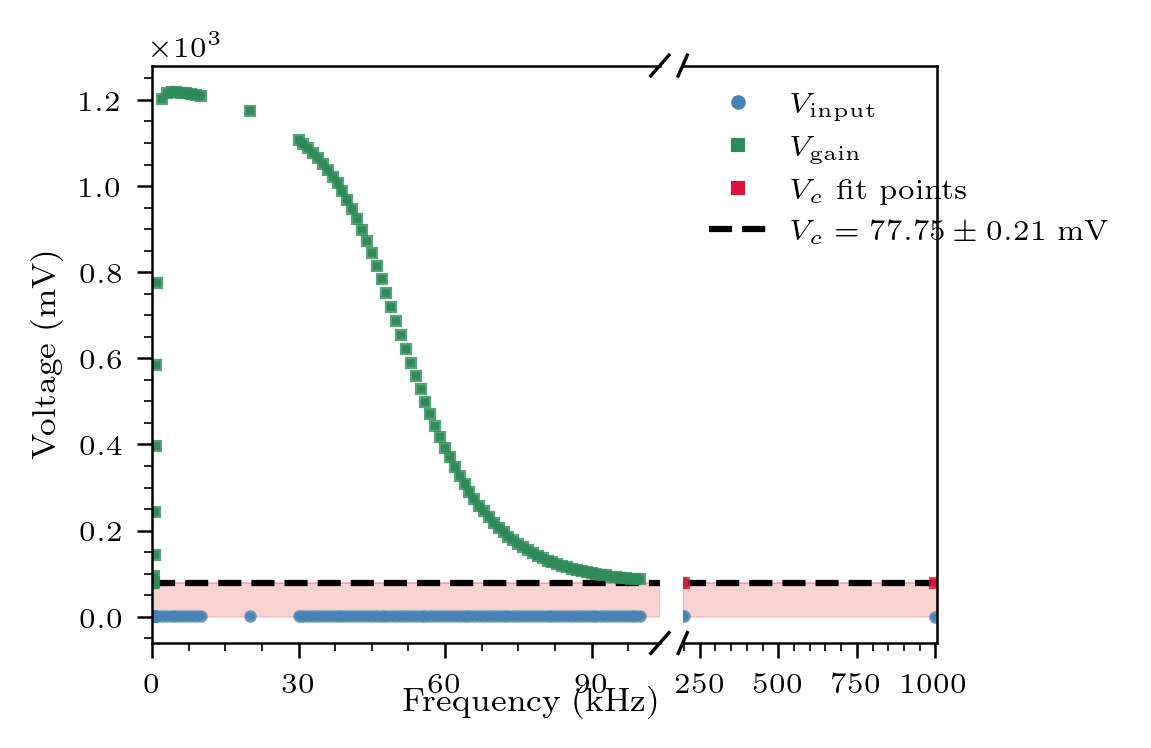
\includegraphics[width=1\linewidth]{calibration_raw.png}
    \caption{Raw data of $V_{\text{gain}}$ (green) and $V_{\text{in}}$ (blue, inner plot)  collected in the calibration stage of the experiment. The constant noise level is highlighted in dashed black and colored light red. Data points which were used to calculate the noise floor are colored red.  }
    \label{fig:calibration_raw}
\end{figure}
Figure \ref{fig:calibration_raw} shows the obtained raw calibration data for $V_{\text{gain}}$ and $V_{\text{in}}$ with estimated statistical uncertainties resulting from the multimeter display values. The maximum gain ratio achieved at frequencies in the kHz range is approximately $10^3$, matching our estimate for the maximum overall apparatus gain. Additionally, $V_{\text{gain}}$ decays characteristically around $50$ kHz, matching our configured low-pass filter range. At high frequencies, $V_{\text{gain}}$ does not converge to $0$, which is the expected behavior for finite $G$, but stabilizes at a constant floor $V_c$, which was obtained by averaging the extremal points at low frequency ($100$ Hz) and high frequency ($200$ kHz, 1 MHz). $V_c$ is later corrected for by subtracting it in quadrature from $V_{\text{gain}}$. 

The inset plot of $V_{\text{in}}$ shows that the signal generator's output voltage does not remain at the configured value of $1$ mV RMS, but deviates from this value by a frequency-dependent amount. This is likely due to the signal generator internally compensating for the impedance of the device under measurement, which is assumed to be the standard $50\ \Omega$; however, the Agilent multimeter has a significantly larger internal impedance of $1\ \text{M}\Omega$ \cite{hewlett_packard_34401a_users_guide_1996}. This impedance mismatch highlights a potential systematic discrepancy between the input voltage actually applied to the photodiode circuit and the measured $V_{\text{in}}$.
\begin{figure}[h]
    \centering
    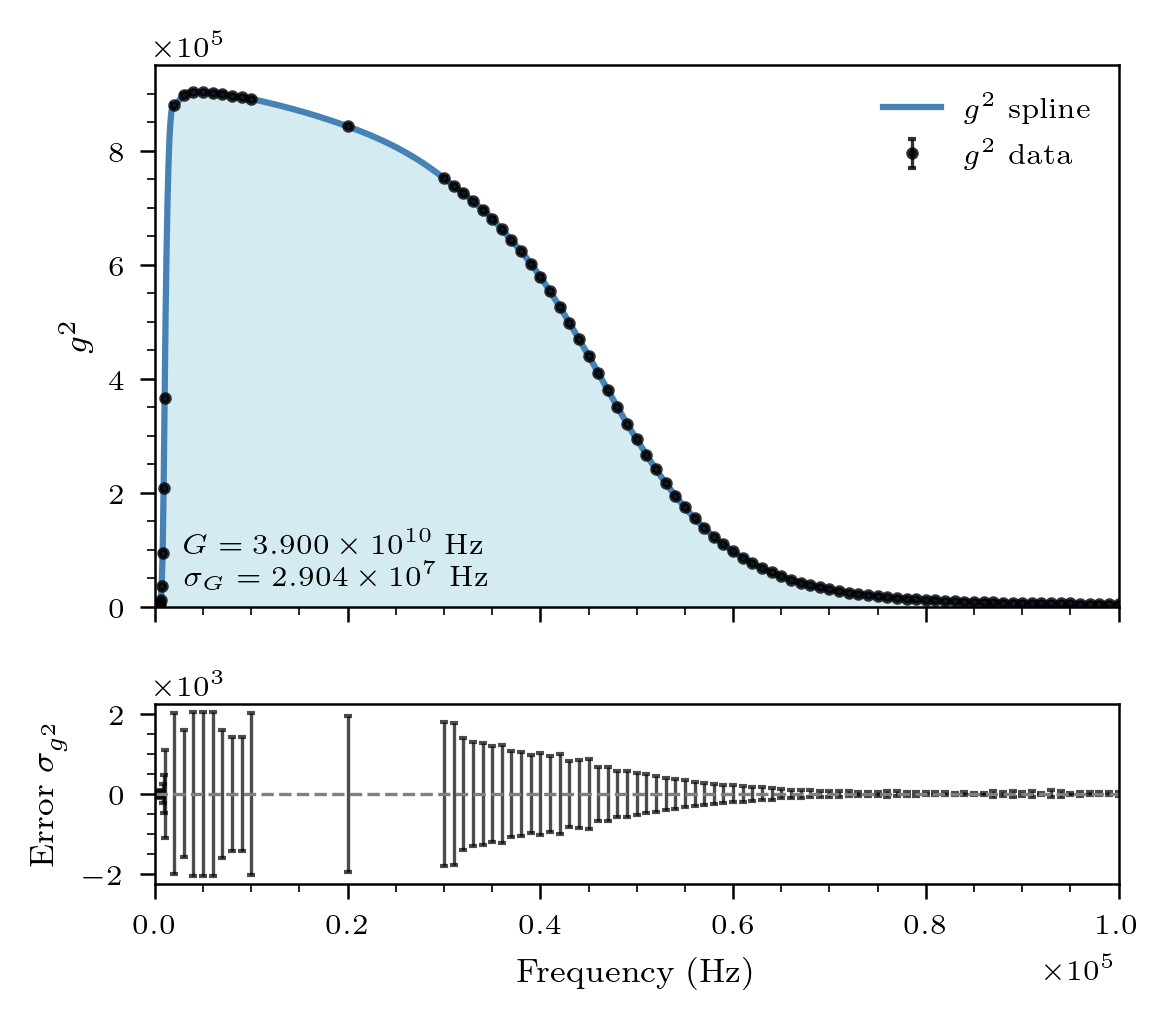
\includegraphics[width=1.0\linewidth]{gain_curve.png}
    \caption{The top plot of the squared gain ratios (black) obtained from \ref{fig:apparatus} versus frequency, which are fit to a cubic spline (dark blue). The bottom plot shows the propagated error magnitude on each data point.}
    \label{fig:gain}
\end{figure}

Proceeding to the calculation of the uncorrected gain integral $G$ as shown in Figure \ref{fig:gain}, the frequency-dependent gain is calculated from the raw data as 
\begin{equation}
    g(f) = \frac{V_{\rm gain}}{ V_{\rm input}}
\end{equation}
and the uncertainty $\sigma_g(f)$ is propagated accordingly.
Figure~\ref{fig:gain} shows a sharply increasing squared gain at low frequencies and a smooth roll-off over the kHz range. The lower panel shows the propagated statistical uncertainty for each data point. A cubic spline is fit to interpolate the trend and is then analytically integrated from $0$ to $100$ kHz to obtain $G$ over this range. The uncertainty $\sigma_G$ is estimated by propagating the uncertainties of each individual data point,
\begin{equation}
    \sigma_G \approx \sqrt{\sum_{i=1}^N\left(\Delta f_i\,\sigma_{g^2_i}\right)^2}
\end{equation}

The obtained values of $G$ and $\sigma_G$ are shown in the figure. To account for gain contributions at higher frequencies, data points from $60$ to $100$ kHz are fit to a power-law model $g^2_{\text{tail}} \propto 1/f^8$. Integrating this tail yields a contribution $G_{\rm tail} = (2.1515 \pm 0.0001) \times 10^7$ Hz, which is three orders of magnitude smaller than $G$, confirming that the contribution of frequencies above $100$ kHz to the gain integral is negligible. The tail model is retained as an order-of-magnitude estimate of the correction to $G$, and its fit uncertainty is propagated as a contribution to the systematic uncertainty in $G$.

\begin{figure}
    \centering
    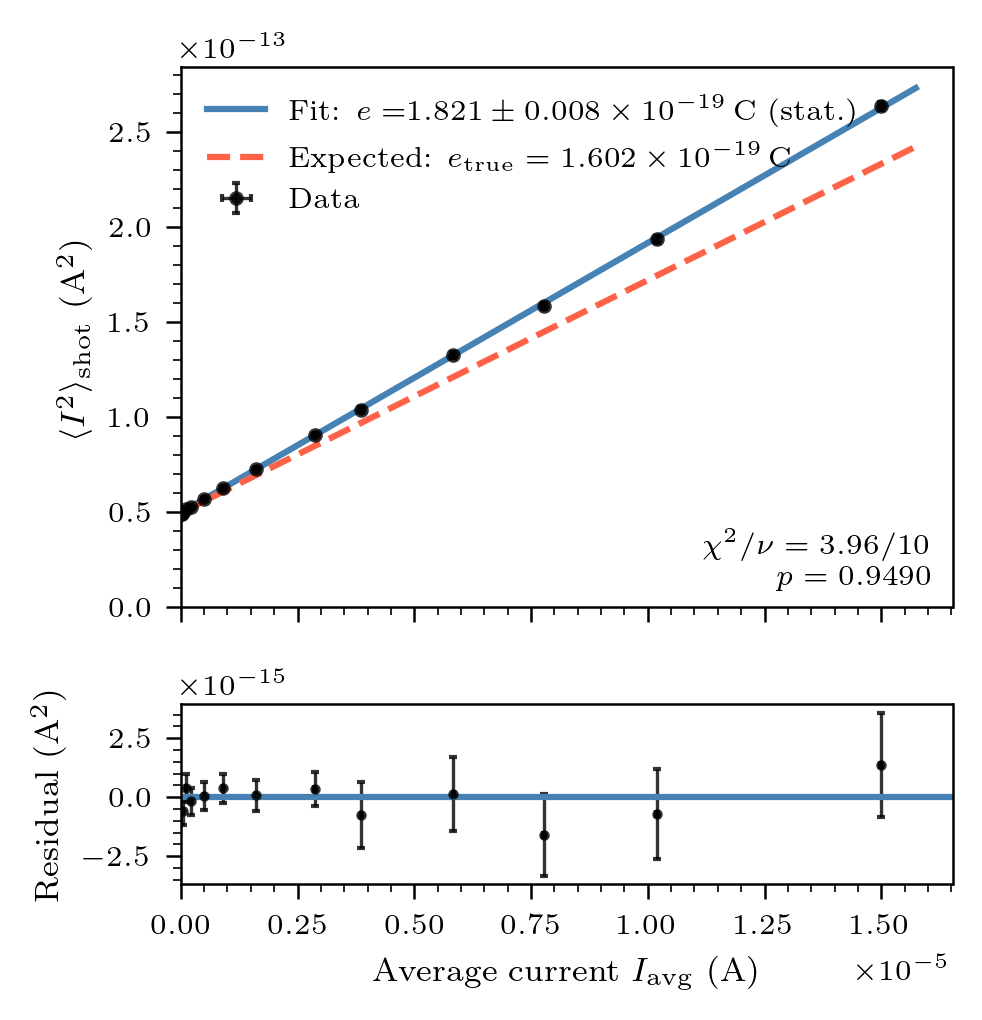
\includegraphics[width=1.0\linewidth]{shot_noise.png}
    \caption{The measured squared shot noise current $\langle I^2 \rangle_{\text{shot}}$ versus average DC current $I_{\text{avg}}$, fit to Eq.~\eqref{eq:shot-noise} with an accompanying residual plot. The uncorrected value of $e$ extracted from the fit is displayed. The expected trend using the accepted value of $e$ is shown as a dashed red line.}
    \label{fig:shot-noise}
\end{figure}

Figure \ref{fig:shot-noise} shows the shot noise experiment results with a plot of the DC current $I_{\text{avg}}$ versus the measured squared mean shot noise current $\langle I^2 \rangle_{\text{shot}}$. These values and their uncertainties were calculated from the measured values and estimated uncertainties of $\langle I^2 \rangle_{\text{shot}}$ and $V_{\text{avg}}$ using the relations
\begin{equation}
    \langle V ^2\rangle_{\text{shot}} = \langle I^2 \rangle_{\rm shot} R_F^2
\end{equation}
\begin{equation}
    V_{\text{avg}} = I_\text{avg} R_F
\end{equation}

Here, we assume that the precision feedback resistor has a standard relative uncertainty of $1$\%. Using SciPy's Orthogonal Distance Regression (ODR) functionality, we fit the trend to the functional form given by \ref{eq:shot-noise} and use the calculated value for $G$ to estimate the uncorrected electron charge $e$. The statistical uncertainty reported from the ODR fit algorithm is taken to be the overall statistical uncertainty in $e$. A low $\chi^2/\text{DOF}$ value and a p-value within the standard range indicate that Eq.~\eqref{eq:shot-noise} is a good fit to the obtained results. The fit quality is further confirmed by the accompanying residual plot, which exhibits no clear systematic trend.

Assuming the accepted value of $e$, an expected trend is plotted alongside the obtained results, showing that $e$ is overestimated by approximately $13.67\%$. To assess the extent to which this discrepancy can be explained by the proposed corrections and estimated uncertainties, we summarize all contributing factors in this analysis:

\begin{table}[h]
\centering
\begin{tabular}{|l|r|r|}
\toprule
\textbf{Source} & \textbf{Value (C)} & \textbf{Rel. to $e$} \\
\midrule
\quad Noise-floor subtraction ($V_c$) & $+3.87 \times 10^{-21}$ & $+2.08\%$ \\
\quad Tail model ($f > 100\,\mathrm{kHz}$) & $-1.05 \times 10^{-22}$ & $-0.06\%$ \\
\midrule
\textbf{Total Correction} & $+3.77 \times 10^{-21}$ & $+2.03\%$ \\
\bottomrule
\end{tabular}
\caption{Systematic corrections applied to the shot-noise measurement of $e$. Here, the raw value and relative magnitude with respect to the original value of $e$ are provided as columns for each error source.}
\label{tab:corrections}
\end{table}

\begin{table}[h]
\centering
\begin{tabular}{|l|r|r|}
\toprule
\textbf{Source} & \textbf{Value (C)} & \textbf{Rel.\ Error} \\
\midrule
\quad Statistical (ODR slope) & $\pm8.02 \times 10^{-22}$ & $\pm0.43\%$ \\
\quad Resistor $R$ (1\% tolerance) & $\pm1.86 \times 10^{-21}$ & $\pm1.00\%$ \\
\quad Gain integral $\mathcal{G}$ & $\pm1.41 \times 10^{-22}$ & $\pm0.08\%$ \\
\quad Tail model ($f > 100\,\mathrm{kHz}$) & $\pm6.42 \times 10^{-26}$ & $\pm0.00\%$ \\
\midrule
\textbf{Total Statistical} & $\pm8.02 \times 10^{-22}$ & $\pm0.43\%$ \\
\textbf{Total Systematic} & $\pm1.86 \times 10^{-21}$ & $\pm1.00\%$ \\
\textbf{Total Uncertainty} & $\pm2.03 \times 10^{-21}$ & $\pm1.09\%$ \\
\bottomrule
\end{tabular}
\caption{Statistical and systematic uncertainties on the shot-noise measurement of $e$. The total uncertainty is obtained by combining the total statistical and systematic uncertainties in quadrature.}
\label{tab:uncertainties}
\end{table}

Applying these corrections and sources of systematic uncertainty to our initial estimate of $e$, we obtain the final result
\begin{equation}
    e = \left( 1.858 \pm 0.008_{\rm stat} \pm 0.019_{\rm sys} \right) \times 10^{{-19}}\,\text{C}
\end{equation}
This indicates that systematic effects, particularly the uncertainty in the precision feedback resistor, constitute the dominant contribution to the total uncertainty in $e$. Combining the statistical and systematic uncertainties in quadrature, our result deviates from the accepted value of $e$ by approximately $12.63\,\sigma$, demonstrating that the corrections and uncertainties accounted for in this study are insufficient to explain the observed discrepancy.

Figure~\ref{fig:shot-noise} suggests that the systematic effect responsible for the deviation maintains a linear dependence on $I_{\text{avg}}$, primarily manifesting as a modification of the slope. The two most plausible forms this error could take are:
\begin{equation}
\langle I^2\rangle_{\rm net}
=
(2eG + \rm Interference)  \,I_{\rm avg}
\label{eg}
\end{equation}
\begin{equation}
\langle I^2\rangle_{\rm net}
=
2e(G + \rm Interference)  \,I_{\rm avg} 
\label{ag}
\end{equation}

In Eq.~\eqref{eg}, the systematic interference enters as a separate contributing noise source, while in Eq.~\eqref{ag} it manifests as an effective modification of the gain integral. A number of potential error sources do not fit either form: Johnson noise, an inherent noise source in any resistive conductor, depends on the resistance $R_F$ but not on $I_{\text{avg}}$ or $G$ and can therefore be ruled out. Another unlikely source is an inaccuracy in the precision feedback resistor. Computing the value of $R_F$ that would reproduce the accepted value $e = 1.602 \times 10^{-19}$ C yields $R_F \approx 550\ \text{k}\Omega$, which deviates from the nominal value of $475\ \text{k}\Omega$ by approximately $13.6\%$, an implausibly large deviation given the stated tolerance of the precision resistor. Future direct measurements of $R_F$ could confirm this reasoning.

The most plausible error source is a calibration-stage mismatch between the measured signal generator voltage $V_\text{in}$ and the actual voltage applied at the ``Test In'' input of the photodiode circuit, which would manifest as an effective modification of $G$ as in Eq.~\eqref{ag}. The signal generator assumes its output is applied across a standard $50\ \Omega$ load, whereas the Agilent multimeter presents a much larger impedance of $1\ \text{M}\Omega$ so as not to draw current from the circuit under measurement. Given that the photodiode circuit input likely presents an impedance closer to $50\ \Omega$, the actual voltage applied to the circuit may be systematically lower than the measured $V_\text{in}$. Lower values of $V_{\text{in}}$ would yield higher gain ratios $g(f)$ and therefore an overestimated $G$, leading to an underestimate of $e$ — consistent with the direction of the observed discrepancy. Another plausible systematic effect of the form given in Eq.~\eqref{eg} is current-dependent shot noise originating from active circuit elements in the amplification chain, such as the operational amplifiers, the preamplifier, or the bandpass filter.



%%%%%%%%%%%%%%%%%%%%%%%%%%%%%%%%%%%%%%%%%%%%%%%%%%%%%%%%%%%%%%%%%%%%%%%%%%%%%


%%%%%%%%%%%%%%%%%%%%%%%%%%%%%%%%%%%%%%%%%%%%%%%%%%%%%%%%%%%%%%%%%%%%%%%%%%%%%
\section{Conclusions}
We report a value for the charge of the electron 
\begin{equation}
    e = \left( 1.858 \pm 0.008_{\rm stat} \pm 0.019_{\rm sys} \right) \times 10^{{-19}}\,\text{C}
\end{equation}
which deviates from the accepted value by approximately $12.63 \ \sigma$. Uncertainties and corrections are summarized in Tables~\ref{tab:corrections} and~\ref{tab:uncertainties}. The agreement between the expected behavior of the gain calibration chain and the obtained calibration data demonstrates that the apparatus is operating largely as designed. The strong quantitative agreement between Eq.~\eqref{eq:shot-noise} and the experimental results provides compelling evidence that electric current exhibits Poissonian shot noise, supporting the hypothesis of the granular nature of electric charge. However, the statistical and systematic uncertainties accounted for in this study are insufficient to explain the $12.63\,\sigma$ discrepancy with the accepted value. Further investigation is therefore required to identify the dominant systematic effects in the apparatus and to obtain a more accurate determination of the electron charge $e$.

%%%%%%%%%%%%%%%%%%%%%%%%%%%%%%%%%%%%%%%%%%%%%%%%%%%%%%%%%%%%%%%%%%%%%%%%%%%%%
\begin{acknowledgments} 
The authors thank Max Misterka for collaboration during the data collection phase of this experiment, and the J-Lab staff for providing the experimental equipment and laboratory manual, as well as for their guidance and technical support throughout. The AI tools ChatGPT and Claude Code were used to assist with literature review and to generate the analysis code and figures used in this paper. The source
code for this paper can be found at \cite{suresh_shot_jlab}.
\end{acknowledgments}

%%%%%%%%%%%%%%%%%%%%%%%%%%%%%%%%%%%%%%%%%%%%%%%%%%%%%%%%%%%%%%%%%%%%%%%%%%%%%
% Place all of the references you used to write this paper in a file
% with the same name as following the \bibliography command
%%%%%%%%%%%%%%%%%%%%%%%%%%%%%%%%%%%%%%%%%%%%%%%%%%%%%%%%%%%%%%%%%%%%%%%%%%%%%

\bibliography{sample-paper}


%%%%%%%%%%%%%%%%%%%%%%%%%%%%%%%%%%%%%%%%%%%%%%%%%%%%%%%%%%%%%%%%%%%%%%%%%%%%%
\clearpage
\end{document}